\section{Einleitung}

Diese Dokumentation soll während des ganzen Projekt ergänzt und nachgeführt werden.
\subsection{Zweck dieser Applikation}
\begin{itemize}
\item Diese App ist für Verkündiger gedacht.
\item Es soll nicht als Ersatz der Dienstabmachungen mit der eigenen Versammlung dienen.
\item Diese App soll lediglich das finden eines Dienstpartners vereinfachen, wenn Verkündiger eine kurzfristige Dienstabsage erhalten oder wenn niemand für den Dienst zu einer bestimmten Zeit gefunden werden konnte.
\item Die App hat ihr Anwendungsgebiet innerhalb einer bestimmten Region, welche im Moment auf den Raum Zürich beschränkt ist. In einem zweiten Schritt könnte die Region mit Wohnort und selbst bestimmten Radius jeder für sich bestimmen.
\item Diese App soll auch Abmachungen mit einer Sprache, die nicht der Muttersprache entspricht, ermöglichen.
\item Der Grundgedanke die Dienstgruppe und die Einheit zu fördern soll bei der Implementierung der Applikation berücksichtigt werden.
\end{itemize}

\subsection{Projektaufbau}

\begin{center}
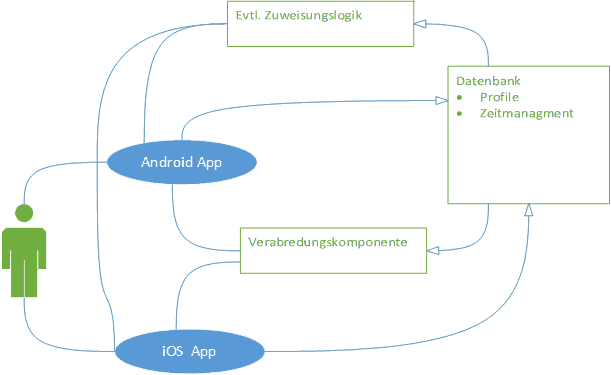
\includegraphics[width=0.75\textwidth]{bilder/useCase.png}
\end{center}
